\chapter{Projektauftrag}

\label{AppendixProjektauftrag}

\section{Ausgangslage}\label{ausgangslage}

Als regelmässiger Konzertbesucher wünsche ich mir eine Plattform im
Internet, auf welcher ich eine zuverlässige Übersicht an Konzerten in
meiner Umgebung vorfinde. Heute sind die Events nur verteilt auf
verschiedenen Seiten wie die der Venues, des Konzertveranstalters, des
Künstlers oder auf Facebook publiziert.

Ich möchte deshalb eine zentrale Plattform entwickeln, die es Benutzern
einfach macht, Konzerte für ihren Geschmack zu finden.

Die Plattform soll Genre unabhängig sein und entsprechende Filter
anbieten.

Um einen zusätzlichen Service für den User zur Verfügungs zu stellen,
ist es auch denkbar, eine Art Notifikationssystem zu bauen um Benutzer
über Handy-Notifications oder per Email an Konzerte oder Künstler zu
erinnern.

Konzertveranstaltern kann das Erfassen ihrer Events vereinfacht werden,
indem auf der Plattform erfasste Veranstaltungen direkt auf den Sozialen
Medien wie Facebook, Twitter oder Instagram geteilt werden können.

\clearpage
\section{Projektziele}\label{projektziele}

\begin{longtable}[]{@{}lll@{}}
  \toprule
  Nr.  & Zielbeschreibung                                                                       & Muss/Kann\tabularnewline
  \toprule
       & Produktziele\tabularnewline
  \midrule
  1.1  & Besucher können im Produkt nach Konzerten suchen                                       & Muss\tabularnewline
  1.2  & Suchresultate können nach Musik-Genre und Ort gefiltert werden                         & Muss\tabularnewline
  1.3  & Das Produkt soll ein modernes responsives Design vorweisen                             & Muss\tabularnewline
  1.4  & Konzerte sollen von Suchmaschinen indexiert werden können                              & Muss\tabularnewline
  1.5  & Benutzer können isch im Produkt registrieren                                           & Muss\tabularnewline
  1.6  & Benutzer können ihr Passwort nach Verlust neu setzen                                   & Muss\tabularnewline
  1.7  & Inhalte des Portals sind durch die Benutzer erfassbar und bearbeitbar                  & Muss\tabularnewline
  1.8  & Kompatibilität mit aktuellem Google Chrome und Mozilla Firefox Browser                 & Muss\tabularnewline
  1.9  & Konzerte können vom Produkt nach Facebook exportiert werden                            & Kann\tabularnewline
  1.10 & Ein angemeldeter Benutzer kann vermerken ob er einem Konzert teilnimmt                 & Kann\tabularnewline
  1.11 & Das Produkt soll sich an Security Best-Practices von OWASP halten                      & Muss\tabularnewline
  \bottomrule
       & Abwicklungsziele\tabularnewline
  \midrule
  2.1  & \makecell[l]{Das Projekt soll nach HERMES 5 unter Berücksichtigung der Richtlinien von                            \\ der TSBE dokumentiert werden} & Muss\tabularnewline
  2.2  & Das Produkt muss bis Projektende fertiggestellt und bereit für die Einführung sein     & Muss\tabularnewline
  2.3  & Die Technische-Umsetzung wird durch Damian Senn erstellt                               & Muss\tabularnewline
  2.4  & \makecell[l]{Die Kommunikation zwischen Experten und Diplomanden erfolgt wie im                                   \\ Projektauftrag \ref{kommunikation} beschrieben.} & Muss\tabularnewline
  2.5  & Das Projekt muss bis Ende Mai 2019 abgeschlossen sein                                  & Muss\tabularnewline
  \bottomrule
\end{longtable}


% TODO: Do I need the following?
%\clearpage
%\subsection{Begründung der
%  Projektziele}\label{begruxfcndung-der-projektziele}

\clearpage
\section{Terminplan}\label{terminplan}

Nachfolgend ist der grobe Terminplan für die geplanten Phasen. Im Anhang~\ref{terminplan} ist
der detaillierte Terminplan abgelegt.

\begin{longtable}[]{@{}lrr@{}}
  \toprule
  Phase           & Datum                   & Stunden\tabularnewline
  \midrule
  \endhead
  Initialisierung & 06.03.2019 - 31.03.2019 & 64\tabularnewline
  Konzept         & 01.04.2019 - 14.04.2019 & 66\tabularnewline
  Realisierung    & 22.04.2019 - 19.05.2019 & 136\tabularnewline
  Abschluss       & 20.05.2019 - 26.05.2019 & 36\tabularnewline
  \midrule
                  & Total:                  & 286\tabularnewline
  \bottomrule
  \caption{Terminplan}
\end{longtable}


\section{Meilensteine}\label{meilensteine}

% TODO: Datum für jeden Meilenstein einfügen

\begin{longtable}[]{@{}llcl@{}}
  \toprule
  Nr.           & Meilenstein                   & KW & Datum\tabularnewline
  \midrule
  \endhead
  1 & Kickoff-Meeting & 10 & \tabularnewline
  2 & Abschluss Phase Initialisierung & 13 & \tabularnewline
  3 & Zwischen-Meeting & 18 & \tabularnewline
  4 & Abschluss Phase Konzept & 16 & \tabularnewline
  5 & Abschluss Phase Realisierung & 20 \tabularnewline
  6 & Abschluss Phase Einführung & 21 \tabularnewline
  7 & Abschluss-Meeting & 22 \tabularnewline
  \bottomrule
  \caption{Meilensteine}
\end{longtable}

\clearpage

\section{Organigramm}\label{organigramm}

\begin{figure}[!htb]
  \centering
  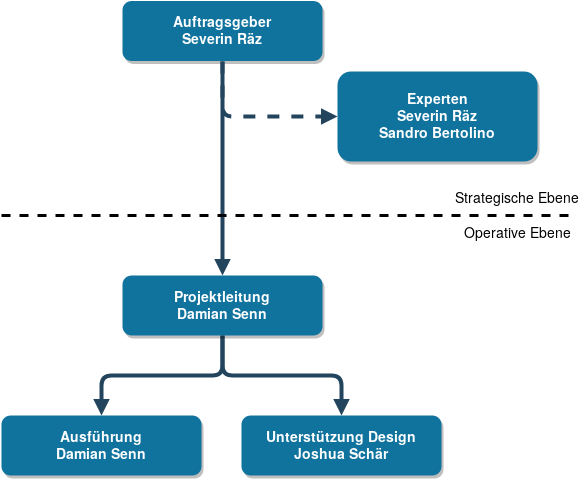
\includegraphics[width=0.8\textwidth]{figures/organigram.png}
  \caption{Organigram}
\end{figure}

\subsection{Tätigkeiten im Projekt}\label{tuxe4tigkeiten-im-projekt}

Für die Freigaben der Phasen ist nach Absprache mit Severin Räz Damian Senn
selbstständig verantwortlich.

\begin{longtable}[]{@{}ll@{}}
  \toprule
  Name             & Funktions- und Tätigkeitsbereich\tabularnewline
  \midrule
  \endhead
  Severin Räz      & Auftraggeber, externer Experte\tabularnewline
  Sandro Bertolino & Interner Experte\tabularnewline
  Damian Senn      & Projektleiter, Ausführung\tabularnewline
  \bottomrule
  \caption{Tätigkeiten Verteilung}
\end{longtable}

\subsection{Kommunikation}\label{kommunikation}

Wie im Kickoff-Meeting besprochen, wird Damian Senn alle zwei Wochen einen
kurzen Bericht an Sandro Bertolino und Severin Räz per E-Mail schicken.
Im Bericht wird erläutert was in der Zwischenzeit erledigt wurde und was
die nächsten Schritte im Projekt sind.

\clearpage

\section{Abgrenzungen}\label{abgrenzungen}

\begin{figure}[!htb]
  \centering
  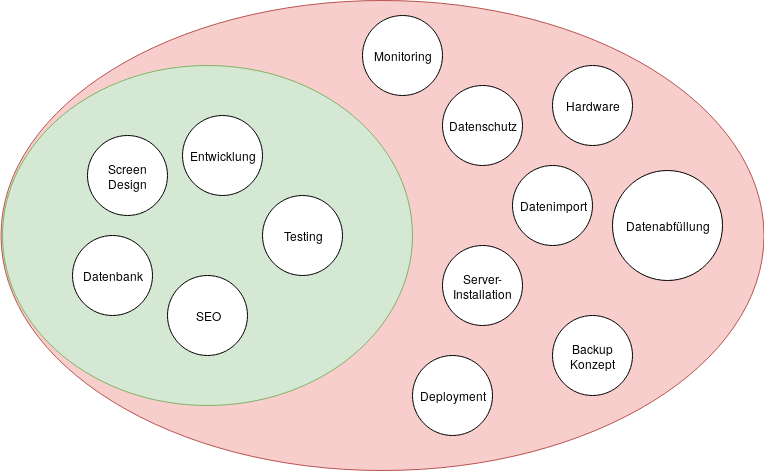
\includegraphics[width=0.95\textwidth]{figures/abgrenzungen.png}
  \caption{Abgrenzungen}
\end{figure}

\subsubsection{Hardware, Server-Installation, Deployment und
  Monitoring}\label{hardware-server-installation-deployment-und-monitoring}

Da das Projekt ein reines Software-Entwicklungs Projekt ist, werden
keine Operativen tätigkeiten wie Hardware beschaffung,
Server-Installation, Deployment und das einrichten eines
Monitoring-Systems vorgenommen.

\subsubsection{Datenschutz}\label{datenschutz}

Da das Projekt nicht deployed wird und somit nicht produktiv/online
gestellt wird, müssen im Rahmen dieser Projektarbeit noch keine Gedanken
über den Datenschutz gemacht werden.

\subsubsection{Datenimport}\label{datenimport}

Da wir bisher keine existierenden Konzertdaten besitzen, ist es nicht
nötig, einen Datenimport zu implementieren.

\subsubsection{Datenabfüllung}\label{datenabfuxfcllung}

Die Projektarbeit beinhaltet kein Datenset, Tests werden mit Testdaten
abgewickelt. Es liegt nicht in der Verantwortung des Projektleiters,
dass Daten in die Applikation abgefüllt werden.

\subsubsection{Backup Konzept}\label{backup-konzept}

Es wird kein Backup Konzept benötigt, da die Applikation im Rahmen
dieses Projektes nicht produktiv geschaltet wird.

\clearpage
\section{Anforderungskatalog}\label{anforderungskatalog}

Der Anforderungskatalog wurde in der Studie erarbeitet. Es wurden Kann und Muss
Kriterien definiert, wobei ein Muss-Kriterium zwingend erfüllt werden muss und
ein Kann-Kriterium als Erweiterung angesehen wird.

% TODO: Fix multirows across pages
%       https://tex.stackexchange.com/questions/79143/how-to-repeat-cell-content-on-next-page-for-longtable-using-multirow/79152
\begin{longtable}[]{@{}p{1.9cm}p{2.5cm}cp{5.5cm}cc@{}}
  \toprule
  \textbf{Feature}           & \textbf{Titel}             & \textbf{Nr.} & \textbf{Kriterium}                                                                                          & \textbf{Ziel} & \textbf{Muss}\tabularnewline
  \midrule
  \endhead
  \multirow{10}{*}{Suche}    & Suche nach Konzertname     & 1.1          & Listet alle Konzerte die Wörter der Suche im Konzertnamen beinhalten                                        & 1.1           & \textbf{Muss}                \\ \cline{2-6}
                             & Suche nach Konzertlocation & 1.2          & Schränkt die Such-Resultate nach gegebener Konzertlocation ein                                              & 1.2           & \textbf{Muss}                \\ \cline{2-6}
                             & Suche nach Ort             & 1.2          & Schränkt die Such-Resultate nach gegebenem Ort ein                                                          & 1.2           & \textbf{Muss}                \\ \cline{2-6}
                             & Suche nach Genre           & 1.2          & Schränkt die Such-Resultate nach gegebenem Musik-Genre ein                                                  & 1.2           & \textbf{Muss}                \\
  \midrule
  \multirow{8}{*}{Design}    & Desktop                    & 2.1          & Alle Ansichten haben eine Desktop-Optimierte Variante                                                       & 1.4           & \textbf{Muss}                \\ \cline{2-6}
                             & Tablet                     & 2.2          & Alle Ansichten haben eine Tablet-Optimierte Variante                                                        & 1.4           & \textbf{Muss}                \\ \cline{2-6}
                             & Mobile                     & 2.3          & Alle Ansichten haben eine Mobile-Optimierte Variante                                                        & 1.4           & \textbf{Muss}                \\ \cline{2-6}
                             & Browser Kompatibilität     & 2.4          & Alle Ansichten müssen in aktuellem Google Chrome und Mozilla Firefox dem Grundlayout folgen                 & 1.9           & \textbf{Muss}                \\
  \midrule
  \multirow{4}{*}{SEO}       & Indexierbarkeit            & 3.1          & Das Produkt ist von Suchmaschinen indexierbar                                                               & 1.5           & \textbf{Muss}                \\ \cline{2-6}
                             & Linked Data                & 3.2          & Konzert Detailseiten sind mit dem Event-Schema\footnote{\url{https://schema.org/Event}} ausgestattet              & 1.5           & \textbf{Muss}                \\
  \midrule
  \multirow{8}{*}{Benutzer}  & Registrierung              & 4.1          & Besucher können sich einen Benutzer registrieren, Benutzernamen und E-Mail Adressen müssen einzigartig sein & 1.6           & \textbf{Muss}                \\ \cline{2-6}
                             & Passwort-Vergessen         & 4.2          & Benutzer können sich einen Passwort-Reset Link anfordern                                                    & 1.7           & \textbf{Muss}                \\ \cline{2-6}
                             & Social                     & 4.3          & Benutzer können auf Konzerten vermerken ob sie Teilnehmen oder nicht                                        & 1.11          & Kann                         \\
  \midrule
  \clearpage
  \multirow{6}{*}{Erfassung} & Artist                     & 5.1          & Benutzer können Artisten mit einem Genre erfassen                                                           & 1.8           & \textbf{Muss}                \\ \cline{2-6}
                             & Location                   & 5.2          & Benutzer können eine Konzertlocation mit Ort/Strasse erfassen                                               & 1.8           & \textbf{Muss}                \\ \cline{2-6}
                             & Konzert                    & 5.3          & Benutzer können ein Konzert mit Konzertlocation und Artisten erfassen                                       & 1.8           & \textbf{Muss}                \\ \cline{2-6}
                             & Facebook                   & 5.4          & Benutzer können ein Konzert in ein Facebook-Event exportieren                                               & 1.10          & Kann                         \\
  \midrule
  \multirow{9}{*}{Security}  & SQL-Injection              & 6.1          & Das Produkt soll resistent gegen SQL-Injection sein                                                         & 1.12          & \textbf{Muss}                \\ \cline{2-6}
                             & HTML-Injection             & 6.2          & Das Produkt soll resistent gegen HTML-Injection / XSS sein                                                  & 1.12          & \textbf{Muss}                \\ \cline{2-6}
                             & Passwort encryption        & 6.3          & Passwörter von Benutzer müssen mit einem sicheren Verfahren gespeichert werden                              & 1.12          & \textbf{Muss}                \\ \cline{2-6}
                             & Session                    & 6.4          & Session-Cookies dürfen nicht durch JavaScript ausgelesen werden                                             & 1.12          & Kann                         \\
  \midrule
  Performance                & Ladezeit                   & 7.1          & Die Seitenansichten dürfen nicht länger als 6 Sekunden auf einem 3G Netz laden                              &               & \textbf{Muss}                \\
  \midrule
  Sonstiges                  & User Tracking              & 8.1          & Benutzerverhalten soll analysiert und nachvollziehbar sein.                                                 &               & Kann                         \\
  \bottomrule
  \caption{Anforderungskatalog}
\end{longtable}


\clearpage
\section{Lösungsbeschreibung}\label{loesungsbeschreibung}

In der Studie (Anhang~\ref{AppendixStudie}) wurden Technologien gegenüber
gestellt und für die Umsetzung mittels Nutzwertanalysen ausgewählt.

Folgende Technologien wurden ausgewählt:

\textbf{Browser sowie Server Technologie:}

\begin{figure}[!htb]
  \centering
  
\includegraphics[width=0.8\textwidth]{figures/phoenix.png}
  \caption{Phoenix Framework}
\end{figure}

\textbf{Testing Technologie:}

\begin{figure}[!htb]
  \centering
  
\includegraphics[width=0.8\textwidth]{figures/wallaby.png}
  \caption{Wallaby}
\end{figure}
